\documentclass[aspectratio=1610]{beamer}
\usepackage[utf8]{inputenc}
\usepackage[T1]{fontenc}
\usepackage[german]{babel}
\usepackage[useregional]{datetime2}
\usepackage[nameinlink]{cleveref}
\usepackage[section]{placeins}
\usepackage{xcolor}
\usepackage{graphicx}
\usepackage{csquotes}
\usepackage{amsmath} % for $\text{}$
\usepackage{enumitem}
\usepackage{entwurf}
\usepackage{algorithm}
\usepackage{algorithmicx}
\usepackage{algpseudocode}
\usepackage{listings}
\usepackage{bera}
\usepackage{pdfpages}

\colorlet{punct}{red!60!black}
\definecolor{background}{HTML}{EEEEEE}
\definecolor{delim}{RGB}{20,105,176}
\colorlet{numb}{magenta!60!black}
\lstdefinelanguage{json}{
    basicstyle=\normalfont\ttfamily,
    numbers=left,
    numberstyle=\scriptsize,
    stepnumber=1,
    numbersep=8pt,
    showstringspaces=false,
    breaklines=true,
    frame=lines,
    backgroundcolor=\color{background},
    literate=
     *{0}{{{\color{numb}0}}}{1}
      {1}{{{\color{numb}1}}}{1}
      {2}{{{\color{numb}2}}}{1}
      {3}{{{\color{numb}3}}}{1}
      {4}{{{\color{numb}4}}}{1}
      {5}{{{\color{numb}5}}}{1}
      {6}{{{\color{numb}6}}}{1}
      {7}{{{\color{numb}7}}}{1}
      {8}{{{\color{numb}8}}}{1}
      {9}{{{\color{numb}9}}}{1}
      {:}{{{\color{punct}{:}}}}{1}
      {,}{{{\color{punct}{,}}}}{1}
      {\{}{{{\color{delim}{\{}}}}{1}
      {\}}{{{\color{delim}{\}}}}}{1}
      {[}{{{\color{delim}{[}}}}{1}
      {]}{{{\color{delim}{]}}}}{1},
}

\setlist{nosep}

\newcommand\urlpart[2]{$\underbrace{\text{\texttt{#1}}}{\text{#2}}$}
\raggedbottom
\crefname{figure}{Abb}{Abb}

\newcommand\producttitle{treff.}
\hypersetup{
	pdftitle={Entwurf: \producttitle},
	bookmarks=true,
}

% header & footer
\usepackage{scrlayer-scrpage}
%\lofoot{\today}
%\refoot{\today}
\pagestyle{scrheadings}

\title{
\includegraphics[width = 50mm]{images/logo_crop.png}}
\subtitle{\huge Entwurf}
\author{Lukas Dippon
	\and Jens Kienle
	\and Matthias Noll
	\and Fabian Röpke
	\and Tim Schmidt
	\and Simon Vögele}

\begin{document}

	\begin{frame}[plain]
	\maketitle
	\end{frame}

%%%%%%%% SERVER %%%%%%%%%%

	\begin{frame}[plain]
        \frametitle{\textbf{Server} -- ERD der Serverdatenbank}
        \begin{figure}[!htb]
            \centering
            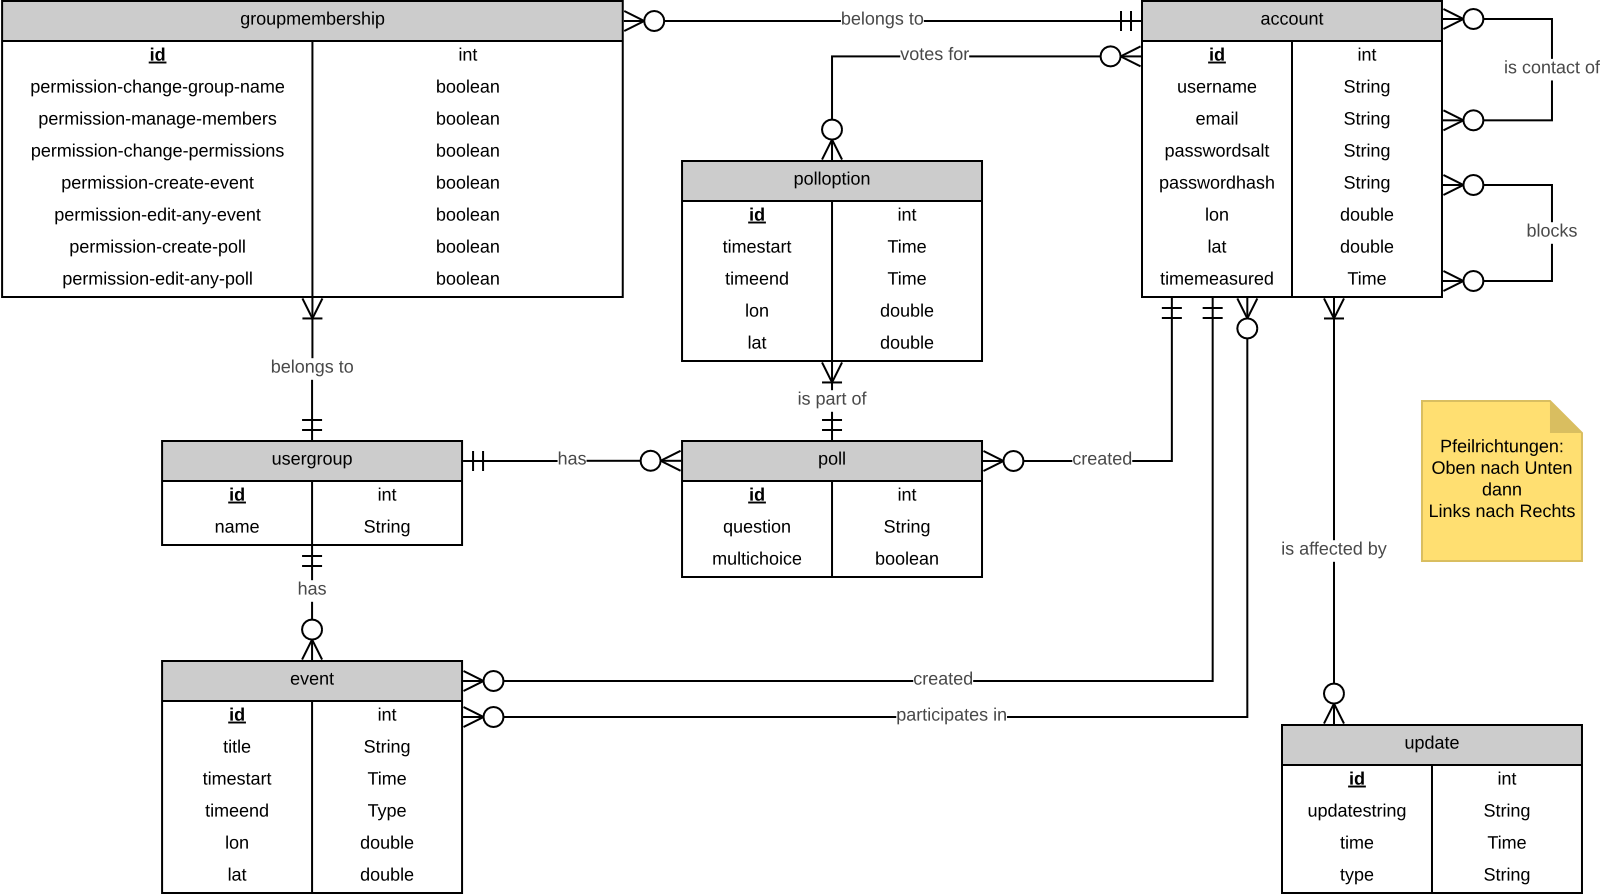
\includegraphics[width = \columnwidth]{images/erd-complete.png}
        \end{figure}
    \end{frame}

	\begin{frame}[plain]
        \frametitle{\textbf{Server} -- Klassen-Diagramm der wichtigsten Klassen}
        \begin{figure}[!htb]
            \centering
            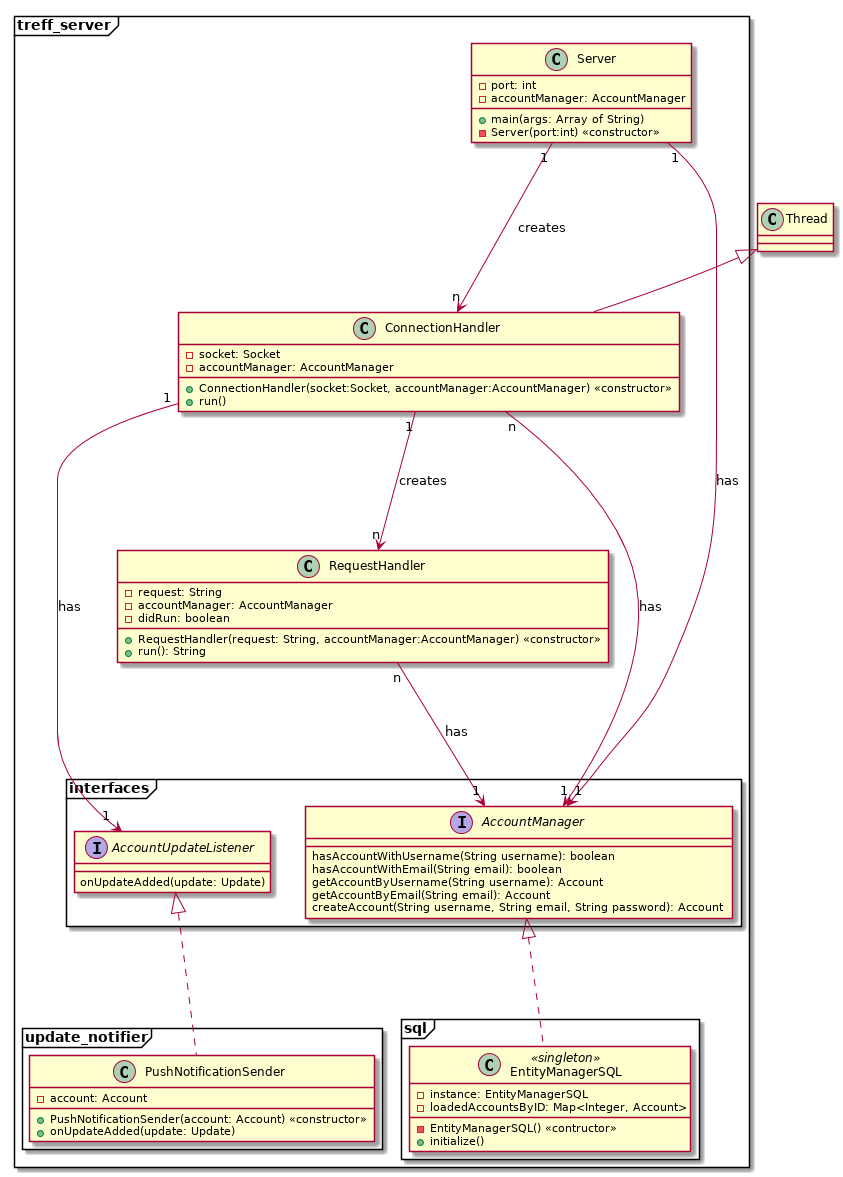
\includegraphics[height = 190pt]{build/uml/server.png}
        \end{figure}
	\end{frame}

	\begin{frame}[plain]
        \frametitle{\textbf{Server} -- Sequenz-Diagramm des Befehls 'get-event-details'}
        \begin{figure}[!htb]
            \centering
            \includegraphics[width = \columnwidth]{build/uml/get-event-details-sequence.png}
        \end{figure}
    \end{frame}

%%%%%%%%% COMM %%%%%%%%%%%

    \apiErrorNew{cred-wrong}{030}{Nutzername/Passwort-Kombination ungültig}
    \apiErrorNew{user-id-invalid}{201}{Mindestens eine
    Benutzerkonto-Identifikationsnummer ungültig}

    \begin{frame}[plain]
        \frametitle{\textbf{Kommunikation} -- Protokoll und Format}
        \begin{minipage}{0.5\textwidth}
            % trim=left bottom right top
            \begin{figure}
                \includegraphics
                [clip, trim=10pt 200pt 140pt 05pt,width=0.95\textwidth]
                {build/listings/login-json.pdf}
                \caption{Request}
            \end{figure}
            \begin{figure}
                \includegraphics
                [clip, trim=10pt 170pt 140pt 05pt,width=0.95\textwidth]
                {build/listings/login-json-response.pdf}
                \caption{Response}
            \end{figure}
        \end{minipage}%
        \begin{minipage}{0.5\textwidth}
            \begin{itemize}
                \item[--] Einfache TCP-Verbindung von Klient zu Server
                \item[--] Verschlüsselt mittels TLS
                \item[--] Mehrere Anfragen pro Verbindung möglich
                \item[--] Befehle im JSON-Format
                    \begin{itemize}
                        \item[$\implies$] menschenlesbar
                        \item[$\implies$] leicht zu implementieren
                        \item[$\implies$] Objekte leicht serialisierbar
                    \end{itemize}
            \end{itemize}
        \end{minipage}
	\end{frame}

    \begin{frame}[plain]
        \frametitle{\textbf{Kommunikation} -- Befehle}
        \only<1>{
            \apiCommand{edit-password}
            {Editieren des eigenen Passworts\\}
            {id/Identifikationsnummer des eigenen Benutzerkontos,
            pass/aktuelles Passwort des eigenen Kontos,
            newpass/vorgeschlagenes{,} neues Passwort}
            {---/Leeres JSON-Objekt bei Erfolg}
            {cred-wrong, user-id-invalid}
        }
        \only<2>{
            \apiCommand{list-groups}
            {Auflisten der Gruppen, in denen das Benutzerkonto Mitglied ist\\}
            {---/Keine weiteren Parameter}
            {groups/Ein Array an oberflächlich beschriebenen Gruppen (siehe
            Kapitel 5.3)}
            {}
        }
	\end{frame}

    \begin{frame}[plain]
        \frametitle{\textbf{Kommunikation} -- Beschreibungen}
            \begin{tabular}[t]{ p{0.2\textwidth} p{0.75\textwidth} }
                \textbf{Oberflächlich}\\
                \hline
                \hfill\textbf{type} & \enquote{group}\\
                \hfill\textbf{id} & Eindeutige Identifikationsnummer der Gruppe{,} mit der diese in
                weiteren Befehlen referenziert werden kann\\
                \hfill\textbf{checksum} & Prüfsumme der ausführlichen
                Beschreibung (siehe 5.10)\\
                \hline\hline
                \textbf{Ausführlich}\\
                \hline
                \hfill\textbf{type} & \enquote{group}\\
                \hfill\textbf{id} & Eindeutige Identifikationsnummer der Gruppe{,} mit der diese in
            weiteren Befehlen referenziert werden kann\\
                \hfill\textbf{name} & Name der Gruppe\\
                \hfill\textbf{members} & Array an
                Identifikationsnummern aller Benutzerkonten, die Mitglied der
                Gruppe sind\\
                \hfill\textbf{events} & Array an oberflächlich
                beschriebenen Verabredungen, die in der Gruppe erstellt worden
                sind (siehe 5.5)\\
                \hfill\textbf{polls} & Array an oberflächlich
                beschriebenen Abstimmungen, die in der Gruppe erstellt worden
                sind (siehe 5.6)\\
            \end{tabular}
	\end{frame}

    \begin{frame}[plain]
        \frametitle{\textbf{Kommunikation} -- Prüfsummen für ausführliche
        Beschreibungen}
        \only<1>{
            \begin{figure}
                % trim=left bottom right top
                \includegraphics
                [clip, trim=10pt 110pt 70pt 05pt,width=0.95\textwidth]
                {build/listings/example-json.pdf}
                \caption{Ausführliche Beschreibung einer Beispielverabredung}
            \end{figure}
        }
        \only<2>{
            \begin{figure}
                % trim=left bottom right top
                \includegraphics
                [clip, trim=05pt 210pt 05pt 05pt,width=0.95\textwidth]
                {build/listings/example-json-normalized.pdf}
                \caption{Ausführliche Beschreibung einer Beispielverabredung}
            \end{figure}
        }
        \only<3>{
            \begin{figure}
                % trim=left bottom right top
                \includegraphics
                [height=230pt]
                {build/uml/synchronize.png}
                \caption{Optimierung der (Re-)Synchronisierung mittels
                Prüfsummen}
            \end{figure}
        }
	\end{frame}

%%%%%%%% CLIENT %%%%%%%%%%

    \begin{frame}[plain]
        \frametitle{\textbf{Klient} -- Layout der HomeActivity}
        \begin{figure}[!htb]
            \centering
            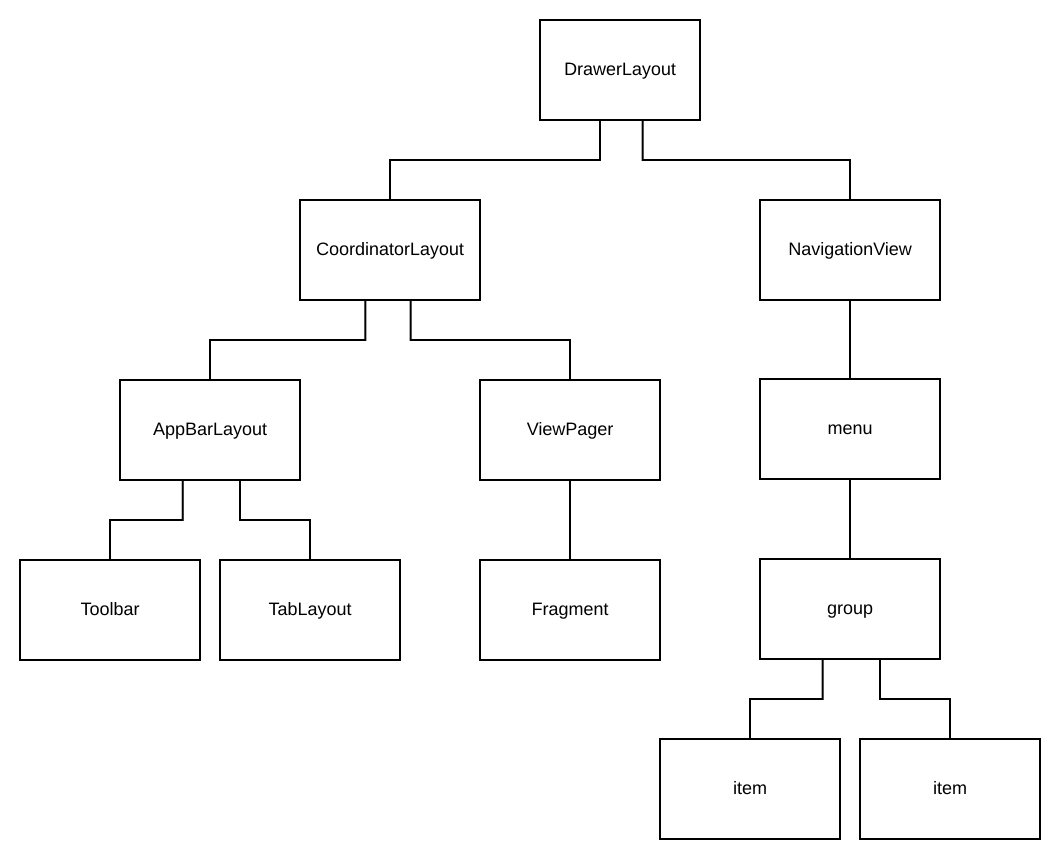
\includegraphics[height = 240pt]{images/activity-home-layout.png}
        \end{figure}
    \end{frame}

	\begin{frame}[plain]
        \frametitle{\textbf{Klient} -- MVVM \& Room am Beispiel der HomeActivity}
        \begin{figure}[!htb]
            \centering
            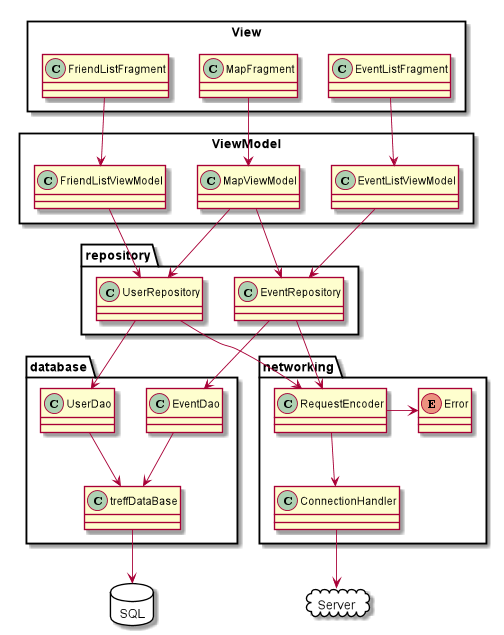
\includegraphics[height = 250pt]{images/database.png}
        \end{figure}
	\end{frame}

    \begin{frame}[plain]
      \frametitle{\textbf{Klient} -- Schnittstelle zum Server}
      \begin{figure}[!htb]
        \centering
        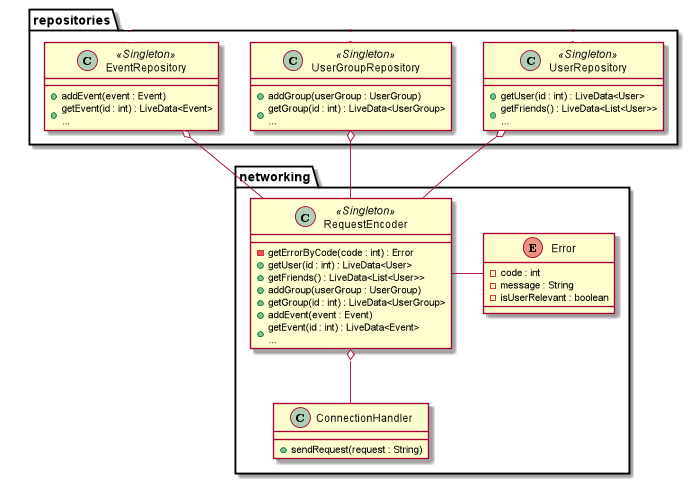
\includegraphics[height = 240pt]{images/connection_client.png}
        \end{figure}
    \end{frame}
    
     \begin{frame}[plain]
      \frametitle{\textbf{Klient} -- Positionsbestimmung}
      \begin{figure}[!htb]
        \centering
        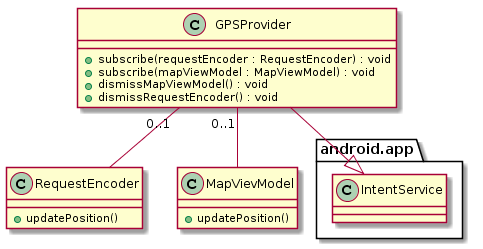
\includegraphics[height = 200pt]{images/gpsprovider.png}
        \end{figure}
    \end{frame}
        
%    \begin{frame}[plain]
%       \frametitle{\textbf{Klient} -- Laden der Freundesliste}
%	      	\begin{figure}[!htb]
%   	    	  \centering
%       	 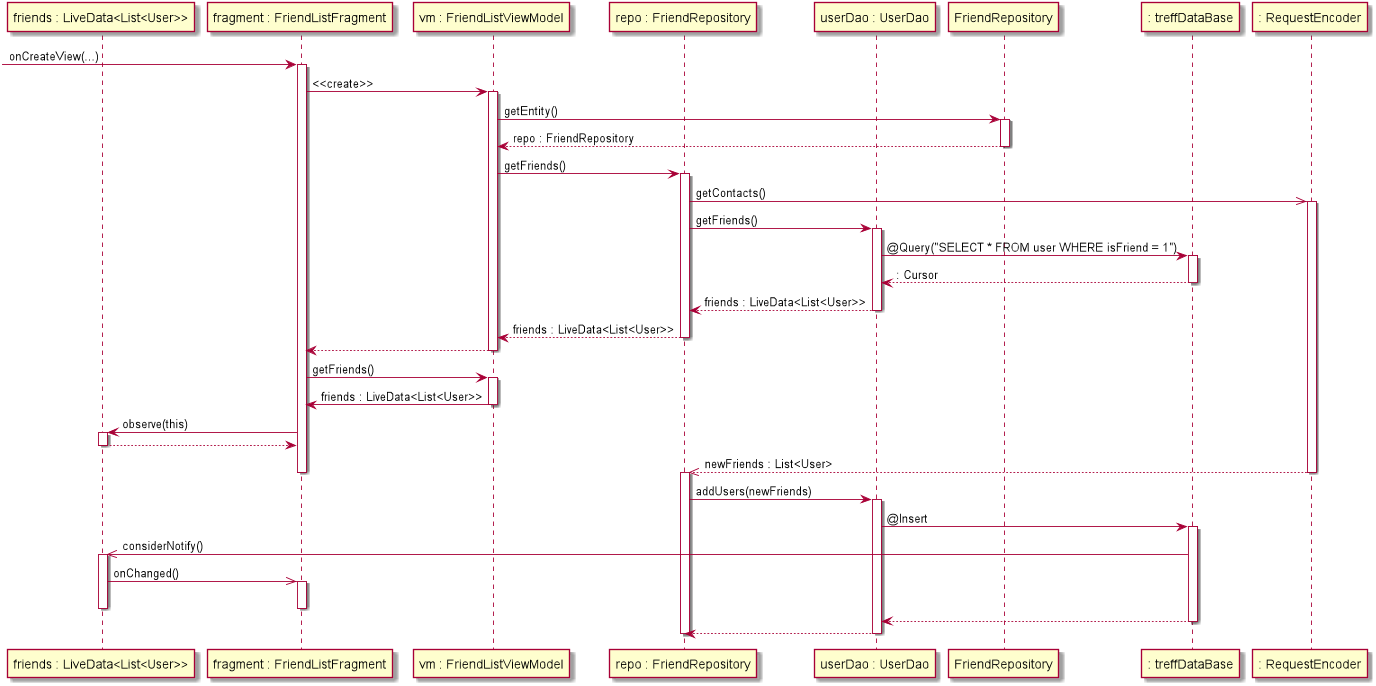
\includegraphics[height = 200pt]{images/datafetch.png}
%   	\end{figure}
% \end{frame}

%%%%%%%%% META %%%%%%%%%%

    \begin{frame}[plain]
        \frametitle{\textbf{Arbeitsweise}}
        \begin{minipage}{0.5\textwidth}
            \only<1>{
        		
\includegraphics[width = \columnwidth - 30pt]
                {images/meet-im-voip.png}
            }
            \only<2>{
        		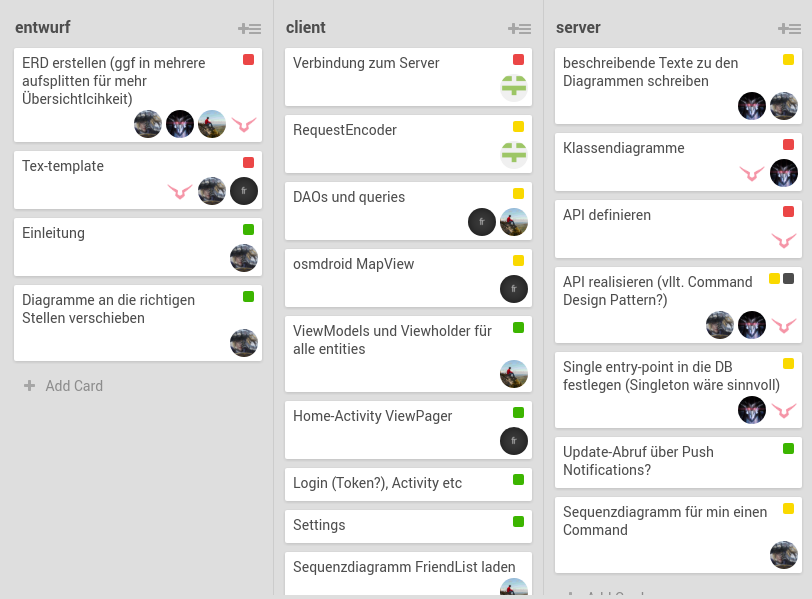
\includegraphics[width = \columnwidth - 10pt]
                {images/kanbanboard-screenshot.png}
            }
            \only<3>{
        		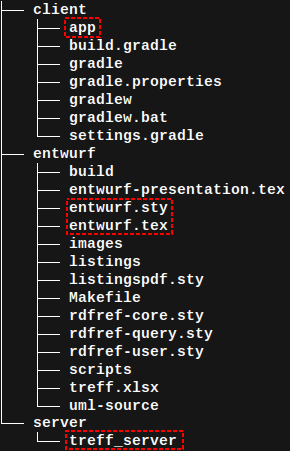
\includegraphics[height = 230pt]
                {images/dir-tree.png}
            }
        	\only<4>{
        		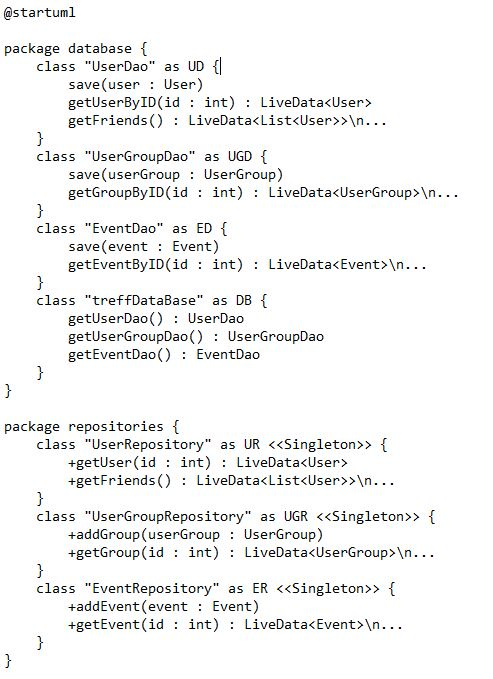
\includegraphics[height = \columnwidth]
        		{images/diagram.JPG}
        	}
        \end{minipage}%
        \begin{minipage}{0.5\textwidth}
            \only<1>{
                \textbf{Kommunikation}
                \begin{itemize}
                    \setlength\itemsep{0.3em}
                    \item[--] Treffen mit allen Gruppenmitgliedern oder in
                        Teilgruppen
                    \item[--] Absprachen über die VoIP-Dienste TeamSpeak und
                        Discord und den Instant Messenger Telegram
                \end{itemize}
            }
            \only<2>{
                \textbf{Aufgabenverteilung und Notizen}
                \begin{itemize}
                    \setlength\itemsep{0.3em}
                    \item[--] Gemeinsame Notizen über Etherpad
                    \item[--] Festhaltung und Zuweisung von Teilaufgaben über
                        ein Kanbanboard	
                \end{itemize}
            }
            \only<3>{
                \textbf{Entwicklung der Struktur und Verfassung des Dokuments}
                \begin{itemize}
                    \setlength\itemsep{0.3em}
                    \item[--] Synchronisierung über Git
                    \item[--] Zwei separate Projekte für Klient und Server
                    \item[--] Entwurfsdokument geteilt in Inhalt (.tex) und
                        Formatierung (.sty)
                \end{itemize}
            }
        	\only<4>{
        		\textbf{Herausforderungen}
        		\begin{itemize}
        			\setlength\itemsep{0.3em}
        			\item[--] Unbekannte Dokumentform
        			\item[--] Differenzen zur Schulung, vieles \enquote{from
        			Scratch}
        			\item[--] Übersichtliche Diagramme erstellen /
        			automatisieren / synchronisieren
        			/ in Formatierung einbinden
        		\end{itemize}
        	}
        \end{minipage}
    \end{frame}
\end{document}
